% ============================================================================
% Diagram sistem kontrol: Kontroler Jaringan Saraf Tiruan / MLP 3-4-1
% Kontrol tekanan pompa via AC chopper. Output NN = ΔDuty (delta), lalu
% diakumulasi (u = u_prev + Δu) -> sifat integral (PI-like).
%
% Cara pakai:
%   1) Compile sendiri: pdflatex diagram_sistem_kontrol.tex  -> hasilkan PDF
%      lalu di skripsi: \includegraphics[width=\textwidth]{gambar/diagram_sistem_kontrol}
%   2) Atau salin isi tikzpicture ke dalam environment figure di bab Anda.
% ============================================================================
\documentclass[border=10pt]{standalone}
\usepackage[utf8]{inputenc}
\usepackage{tikz}
\usetikzlibrary{positioning,arrows.meta,calc,fit,backgrounds}

\begin{document}
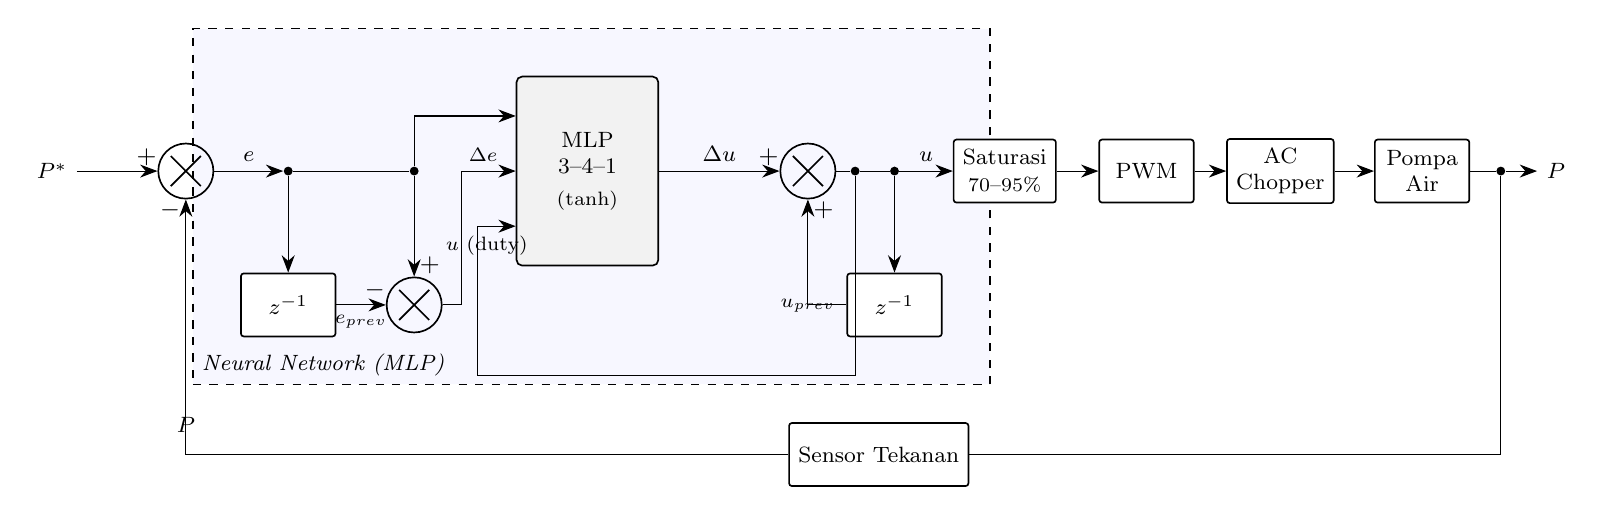
\begin{tikzpicture}[
  font=\footnotesize,
  >={Stealth[length=2.2mm]},
  block/.style={draw, semithick, rounded corners=1pt, minimum height=8mm,
                minimum width=12mm, align=center, fill=white},
  nn/.style={draw, semithick, rounded corners=2pt, minimum height=24mm,
             minimum width=18mm, align=center, fill=black!5},
  sum/.style={draw, semithick, circle, minimum size=7mm, inner sep=0pt,
    path picture={%
      \draw[semithick] ([shift={( 45:2.7mm)}]path picture bounding box.center)
                    -- ([shift={(225:2.7mm)}]path picture bounding box.center);
      \draw[semithick] ([shift={(135:2.7mm)}]path picture bounding box.center)
                    -- ([shift={(315:2.7mm)}]path picture bounding box.center);}},
  dot/.style={circle, fill, minimum size=3.2pt, inner sep=0pt},
  sgn/.style={font=\small}
]

% ---------- node utama (garis maju, y = 0) ----------
\node                (in)  at (0,0)       {$P^{*}$};
\node[sum]           (s1)  at (1.7,0)     {};
\node[dot]           (eb)  at (3.0,0)     {};
\node[dot]           (eb2) at (4.6,0)     {};
\node[nn]            (nn)  at (6.8,0)     {MLP\\ 3--4--1\\[2pt]\scriptsize (tanh)};
\node[sum]           (s3)  at (9.6,0)     {};
\node[dot]           (uf)  at (10.2,0)    {};
\node[dot]           (ud)  at (10.7,0)    {};
\node[block]         (sat) at (12.1,0)    {Saturasi\\\scriptsize $70$--$95\%$};
\node[block]         (pwm) at (13.9,0)    {PWM};
\node[block]         (chop)at (15.6,0)    {AC\\ Chopper};
\node[block]         (pump)at (17.4,0)    {Pompa\\ Air};
\node[dot]           (pb)  at (18.4,0)    {};
\node                (out) at (19.1,0)    {$P$};

% ---------- cabang hitung Delta-e ----------
\node[block] (z1) at (3.0,-1.7) {$z^{-1}$};
\node[sum]   (s2) at (4.6,-1.7) {};

% ---------- akumulator (Delta u -> u) ----------
\node[block] (z2) at (10.7,-1.7) {$z^{-1}$};

% ---------- sensor (umpan balik) ----------
\node[block] (sensor) at (10.5,-3.6) {Sensor Tekanan};

% ---------- garis maju ----------
\draw[->] (in)  -- (s1);
\draw[->] (s1)  -- node[above]{$e$} (eb);
\draw     (eb)  -- (eb2);
\draw[->] (eb2) |- ($(nn.west)+(0,0.7)$);                 % e  -> input atas NN
\draw[->] (nn)  -- node[above]{$\Delta u$} (s3);
\draw     (s3)  -- (uf);
\draw     (uf)  -- (ud);
\draw[->] (ud)  -- node[above]{$u$} (sat);
\draw[->] (sat) -- (pwm);
\draw[->] (pwm) -- (chop);
\draw[->] (chop)-- (pump);
\draw     (pump)-- (pb);
\draw[->] (pb)  -- (out);

% ---------- cabang Delta-e ----------
\draw[->] (eb)  -- (z1);
\draw[->] (z1)  -- node[below]{\scriptsize$e_{prev}$} (s2);   % e_prev -> s2 (-)
\draw[->] (eb2) -- (s2);                                       % e      -> s2 (+)
\draw[->] (s2)  -- (5.2,-1.7) |- ($(nn.west)+(0,0)$)
            node[pos=0.7,above]{\scriptsize$\Delta e$};        % Delta e -> input tengah NN

% ---------- umpan balik u ke NN (input ke-3) ----------
\draw[->] (uf) -- (10.2,-2.6) -- (5.4,-2.6) -- (5.4,-0.7)
            -- ($(nn.west)+(0,-0.7)$)
            node[pos=0.25,below]{\scriptsize$u$ (duty)};

% ---------- akumulator ----------
\draw[->] (ud) -- (z2);
\draw[->] (z2) -- (9.6,-1.7) -- (s3.south)
            node[pos=0.15,below]{\scriptsize$u_{prev}$};

% ---------- umpan balik tekanan ----------
\draw     (pb)     -- (18.4,-3.6) -- (sensor.east);
\draw[->] (sensor.west) -- (1.7,-3.6) -- (s1.south)
            node[pos=0.05,above]{$P$};

% ---------- tanda + / - di sebelah panah (tidak mepet ke lingkaran) ----------
\node[sgn] at ($(s1)+(-0.50,0.18)$)  {$+$};   % P* (panah kiri)
\node[sgn] at ($(s1)+(-0.20,-0.50)$) {$-$};   % umpan balik (panah bawah)
\node[sgn] at ($(s2)+(-0.50,0.18)$)  {$-$};   % e_prev (panah kiri)
\node[sgn] at ($(s2)+(0.20,0.50)$)   {$+$};   % e (panah atas)
\node[sgn] at ($(s3)+(-0.50,0.18)$)  {$+$};   % Delta u (panah kiri)
\node[sgn] at ($(s3)+(0.20,-0.50)$)  {$+$};   % u_prev (panah bawah)

% ---------- kotak putus-putus: controller ----------
\begin{scope}[on background layer]
  \node[draw, dashed, semithick, inner sep=6mm, fill=blue!3,
        fit=(eb)(z1)(s2)(nn)(s3)(z2)(ud)] (ctrl) {};
\end{scope}
\node[anchor=south west, font=\footnotesize\itshape]
      at (ctrl.south west) {Neural Network (MLP)};

\end{tikzpicture}
\end{document}
